\section{Method}
\label{sec:method}

We build the framework around two observations. Because the background is
shared across classes and carries no label-relevant information, the model
needs a reliable way to locate the action; because the classes differ in how
the body moves, the model must also capture the motion at both short and long
time scales. The framework, shown in Figure~\ref{fig:arch}, assigns these
needs to three cooperating branches: a frozen CLIP encoder that locates the
action, a spatio-temporal guidance (STG) block that transfers this knowledge
to the recognition branch, and a temporal action encoder, built on a 2D
ResNet backbone, that models the motion through its dual-granularity temporal
dynamics (DG-TDM) module. Figure~\ref{fig:stg} zooms in on the two core
blocks, STG and DG-TDM.

The data flow is as follows. Given $T$ sampled frames, the frozen CLIP
encoder extracts a patch map from each frame, and a lightweight alignment
module adapts it to the resolution of every backbone stage. The lower branch
is the recognition path: the 2D backbone extracts features stage by stage,
and after each of the four stages the STG block injects the aligned prior
into the features through bilateral window cross-attention, while the DG-TDM
module, inserted after the last bottleneck of the stage, adds temporal
modeling on the 2D feature stream. The final
stage feature is pooled and classified. The three branches divide the work
clearly: the frozen expert answers where the action is, the guidance decides
how much of this knowledge each position receives, and the temporal encoder
models how the action moves. The rest of this section details each part.

\begin{figure}[t]
  \centering
  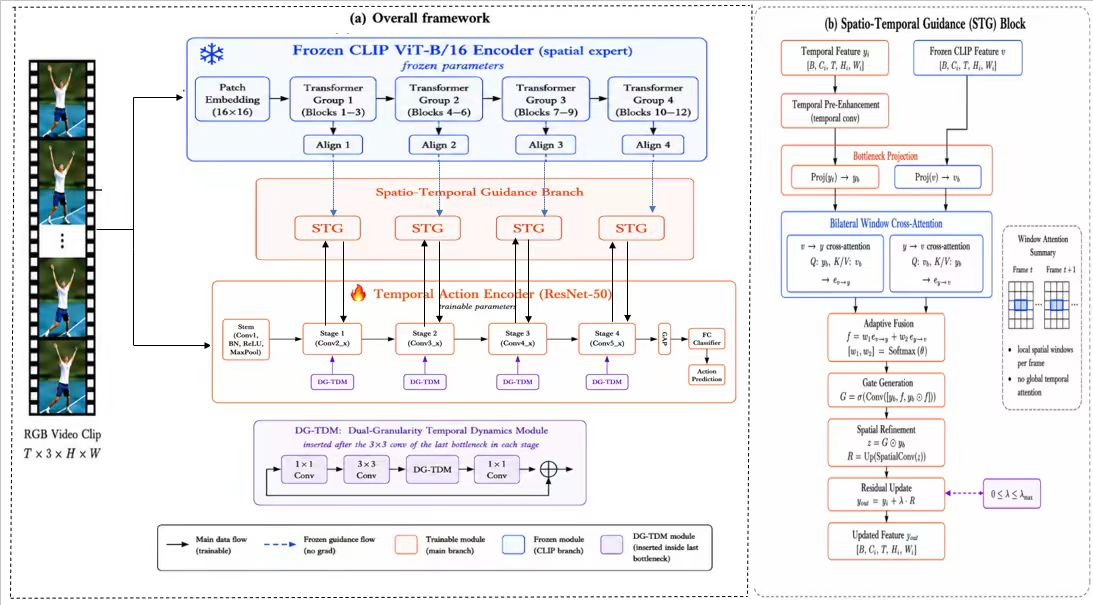
\includegraphics[width=\linewidth]{figures/dgtdm_stg_detail.jpg}
  \caption{Left: the dual-granularity temporal dynamics module (DG-TDM),
  composed of the MoDeA branch (motion deformation attention) and the TSA
  branch (temporal state aggregation). Right: the STG block with bilateral
  window cross-attention, adaptive fusion, and gated refinement.}
  \label{fig:stg}
\end{figure}

\noindent\textbf{Notation.}
Let a video be sampled into $T$ frames and processed by a 2D backbone with
$L$ stages. At stage $\ell$, the lower branch produces a feature map
$Y_\ell \in \mathbb{R}^{B \times C_\ell \times T \times H_\ell \times W_\ell}$,
where $B$ is the batch size and $(H_\ell, W_\ell)$ is the spatial resolution.
The frozen CLIP encoder produces a patch map
$V \in \mathbb{R}^{B \times 768 \times T \times 14 \times 14}$ that is aligned
to each stage resolution by a lightweight projection
$\mathrm{AuxAlign}_\ell(\cdot)$, yielding
$V_\ell \in \mathbb{R}^{B \times C_\ell \times T \times H_\ell \times W_\ell}$.
We use $\odot$ for element-wise multiplication and $\oplus$ for residual
addition, $\mathrm{DWConv}_T$ for a depth-wise convolution along time, and
$\mathrm{GAP}_{hw}$ for global average pooling over the spatial dimensions.

\subsection{Spatial prior and spatio-temporal guidance}
\label{sec:stg}

\textbf{Spatial prior.}
The upper branch is a frozen CLIP ViT-B/16 encoder \cite{radford2021clip}.
What we use is not object semantics but the spatial-position discriminability
acquired during pre-training: the encoder learns where humans, body parts,
and action-relevant objects tend to appear, and can judge, at each location,
whether the content belongs to the action or the background. The encoder
operates frame-wise: each frame passes through the ViT independently, the
class token is discarded, and the patch tokens form a 768-dimensional patch
map $V$ of resolution $14\times 14$. Since the encoder is frozen, this
positional knowledge enters as a stable prior that cannot be distorted by the
limited fine-grained training set. To make the prior available at every
stage, a lightweight alignment module $\mathrm{AuxAlign}_\ell$ interpolates
$V$ to
$(T, H_\ell, W_\ell)$ and applies a $1\times1\times1$ convolution, batch
normalization, and ReLU; the aligned prior $V_\ell$ feeds the guidance branch
below, and these alignment modules are the only trainable parameters attached
to the frozen encoder.

\textbf{Spatio-temporal guidance.}
The STG block is inserted after each temporal stage. Its purpose is to make
the lower branch attend to the action regions that the frozen encoder
identifies, so that the lower branch is not distracted by the background. We
use bilateral window cross-attention: information flows both from the prior
into the lower branch and from the lower branch into the prior, so that the
fusion is a mutual refinement rather than a one-way injection
(Figure~\ref{fig:stg}, right).

Given the lower-branch feature $Y_\ell$ and the aligned prior $V_\ell$, the STG
block first applies a light temporal convolution to $Y_\ell$ to pre-enhance
temporal cues, then projects both inputs into a shared bottleneck dimension
$C_\ell / r$ through separate $1\times1\times1$ convolutions:
\begin{equation}
  Y_b = \mathrm{Conv}^{1}_\mathrm{down}(Y_\ell), \qquad
  V_b = \mathrm{Conv}^{1}_\mathrm{down}(V_\ell).
\end{equation}
The projection to a lower dimension reduces the cost of the subsequent
attention and forces the two inputs to share a compact representation before
interaction.

We then compute bilateral window cross-attention within each local spatial
window. The window operation is confined to $w\times w$ neighborhoods in every
frame and never mixes across time, which keeps the cost linear in the spatial
resolution and preserves per-frame spatial structure: the feature is reshaped
into non-overlapping windows, the attention is applied inside each window, and
the result is restored to the original layout.

The first direction, $V \to Y$, treats $Y_b$ as queries and $V_b$ as keys and
values, letting the lower branch query the frozen prior:
\begin{equation}
  e_{V\to Y} = \mathrm{Softmax}\Big(\frac{Q_{Y} K_{V}^\top}{\sqrt{d}}\Big) V_{V},
  \qquad
  Q_{Y} = Y_b W_Q,\; K_{V} = V_b W_K,\; V_{V} = V_b W_V,
\end{equation}
where $W_Q, W_K, W_V$ are the query, key, and value projections and $d$ is the
head dimension. The second direction, $Y \to V$, reverses the roles and lets
the prior query the lower branch, so that the guidance reflects what the lower
branch has already learned:
\begin{equation}
  e_{Y\to V} = \mathrm{Softmax}\Big(\frac{Q_{V} K_{Y}^\top}{\sqrt{d}}\Big) V_{Y},
  \qquad
  Q_{V} = V_b W_Q,\; K_{Y} = Y_b W_K,\; V_{Y} = Y_b W_V.
\end{equation}
Multi-head attention is applied in both directions, with the query, key, and
value split across heads so that each head can attend to a different aspect of
the interaction.

The two directional outputs are combined by a learned softmax-weighted fusion
to adaptively balance the contribution of each direction. Rather than a fixed
average, we let the network learn the relative weight of the two directions,
which allows the guidance to be dominated by the prior when the lower branch
is uncertain and by the lower branch when it has learned reliable features:
\begin{equation}
  [w_1, w_2] = \mathrm{Softmax}(\beta), \qquad
  f = w_1 \, e_{V\to Y} + w_2 \, e_{Y\to V},
\end{equation}
where $\beta \in \mathbb{R}^2$ is initialized so that $w_1 = w_2 = 0.5$. A
gating network then decides, per spatial position, how much of the fused prior
should be applied to the lower branch. The gate takes the concatenation of
$Y_b$, the fused feature $f$, and their element-wise product, and outputs a
value in $(0,1)$:
\begin{equation}
  G = \sigma\big(\mathrm{Conv}\big([\,Y_b,\; f,\; Y_b \odot f\,]\big)\big).
\end{equation}
Including the product term $Y_b \odot f$ gives the gate access to the
interaction between the two inputs, enabling it to suppress positions where
they disagree. The gate is initialized with a negative bias, so that the
guidance is weak early in training and the lower branch can stabilize first.
The gated feature is refined by a spatial convolution and up-projected back to
the stage channel count, then added to the lower-branch feature with a bounded
residual scale $\lambda \in [0, \lambda_{\max}]$:
\begin{equation}
  \tilde{Y}_\ell = Y_\ell + \lambda \cdot \mathrm{Up}\big(G \odot Y_b\big).
\end{equation}
The scale $\lambda$ is a learnable scalar parameterized through a logit so
that it stays within $[0, \lambda_{\max}]$; it is initialized small to preserve
the identity at the start of training.

\subsection{Dual-granularity temporal dynamics module}
\label{sec:dgtdm}

\begin{figure}[t]
  \centering
  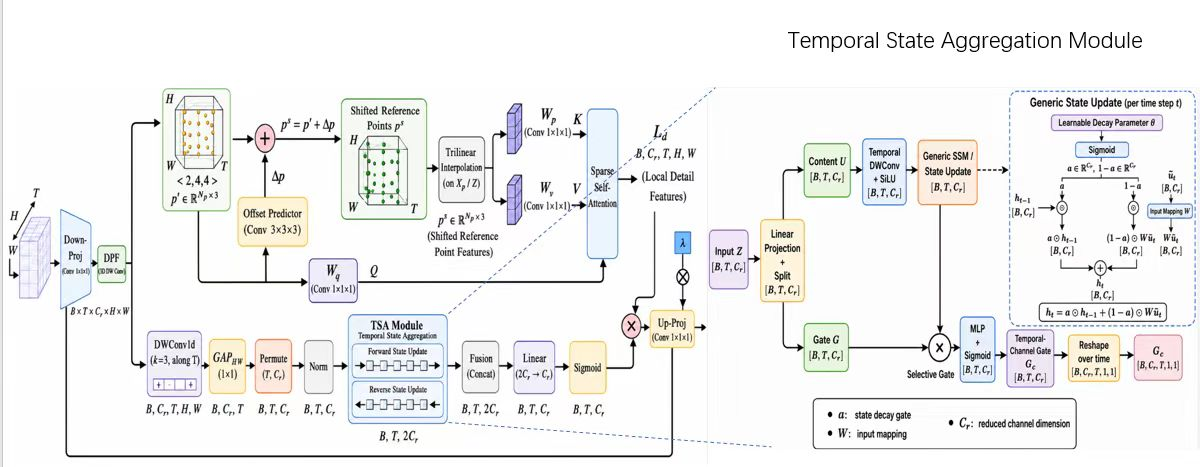
\includegraphics[width=\linewidth]{figures/arch_overview.jpg}
  \caption{Overall framework of \dgtdm. A frozen CLIP encoder extracts spatial
  priors from each frame; the spatial-temporal guidance (STG) branch injects
  these priors into a temporal action encoder through bilateral window
  cross-attention and adaptive gating. Inside each temporal stage, the
  dual-granularity temporal dynamics module (DG-TDM) refines the feature with a
  motion deformation attention (MoDeA) branch and a temporal state aggregation
  (TSA) branch.}
  \label{fig:arch}
\end{figure}

The lower branch is a temporal action encoder built on a 2D ResNet backbone.
A 2D backbone computes the feature of each frame independently and has no
temporal modeling of its own; rather than inflating it into a 3D network, we
insert the dual-granularity temporal dynamics module (DG-TDM)
(Figure~\ref{fig:stg}, left) after the $3\times3$ convolution of the last
bottleneck in each of the four stages. DG-TDM is a pseudo-temporal module: it
does not process frames jointly like a 3D convolution, but injects temporal
dynamics into the 2D features through deformable cross-frame sampling and a
temporal state scan, leaving the backbone structure and its pretrained weights
intact. The module models the motion at the two time scales identified in the
introduction. MoDeA handles the short-term part: it predicts where to sample
across frames to follow the displacement of a body part over successive
frames. TSA handles the long-term part: it carries a state over the whole
sequence and models how the overall temporal response of the action develops.
Together they let the lower branch represent the fine movements that
distinguish fine-grained actions.

\subsubsection{Adapter-style formulation}
\label{sec:adapter}

Following an adapter-style residual design, the DG-TDM block first projects the
stage feature into a compact bottleneck dimension $C_\ell / r$, then applies
the two motion branches, and finally projects back and adds a residual. To
preserve the identity at initialization, the output projection is zero-initialized
and a learnable scalar scale is applied. The structure is
\begin{align}
  X_d &= \mathrm{Down}(X), \label{eq:down}\\
  X_p &= X_d + \mathrm{DPE}(X_d), \label{eq:dpe}\\
  L_d &= X_p + \mathrm{MoDeA}\big(\mathrm{LN}(X_p)\big), \label{eq:modelocal}\\
  \tilde{G}_c &= \mathrm{TSA}\big(\mathrm{GAP}_{hw}\circ \mathrm{DWConv}_T(X_p)\big),
       \label{eq:tsagate}\\
  \tilde{X} &= X + s \cdot \mathrm{Up}\big(\tilde{G}_c \odot L_d\big),
       \label{eq:adapterout}
\end{align}
where $\mathrm{Down}$ and $\mathrm{Up}$ are $1\times1\times1$ convolutions,
$\mathrm{DPE}$ is a depth-wise $3\times3\times3$ convolution that injects
dynamic position information, $\mathrm{LN}$ is layer normalization applied per
spatial--temporal position, $\mathrm{DWConv}_T$ is a depth-wise convolution
along time, $\mathrm{GAP}_{hw}$ is global average pooling over the spatial
dimensions, and $s$ is the learnable scale. We describe $\mathrm{MoDeA}$ and
$\mathrm{TSA}$ next.

The bottleneck design keeps the DG-TDM cheap: the two motion branches operate
in $C_\ell / r$ channels rather than $C_\ell$, and the output projection is
zero-initialized so that the block behaves as an identity at the start of
training. This is important for fine-grained tasks because it lets the
pretrained backbone be reused directly and adds only a small trainable
footprint; it also stabilizes early optimization, since the block initially
passes the stage feature through unchanged and only gradually learns to add
motion-aware refinements. The two branches read the same projected input
$X_p$ but in different ways: MoDeA operates on the full spatio-temporal
tensor and refines it locally, while TSA pools the spatial dimensions first
and returns a compact per-channel gate. The gate is applied to the MoDeA
output $L_d$ before the up-projection, so the two branches interact as a
product: the local motion details are kept only where the temporal memory
indicates that the channel matters for the action.

\subsubsection{Motion deformation attention (MoDeA)}
\label{sec:modela}

Actions are, by definition, movements of body parts relative to one another:
a hand travels from the upper-left corner of the frame to somewhere else, and
the trajectory of that movement is what distinguishes one action from another.
A key consequence is that the position of the action content is \emph{not}
fixed across frames: the location that carries the discriminative detail at
time $t$ holds different, irrelevant content by time $t+1$. A feature sampled
on a fixed grid therefore loses the motion, because it keeps sampling the same
coordinates while the content has moved away. MoDeA addresses this by
predicting, at each spatio-temporal position, a deformation offset that tracks
where the relevant content has moved, and then attending over the displaced
sampling positions. This follows the line of deformable video transformers
\cite{dvt2022}, which select the patches to attend based on motion, but differs
in that MoDeA predicts a dense 3D offset field and performs continuous
trilinear sampling, giving a finer representation of local motion than
patch-level selection.

Formally, let $Z = \mathrm{LN}(X_p)$ denote the layer-normalized input of
shape $[B, C_r, T, H, W]$, where $C_r = C_\ell / r$. The branch first projects
the query from $Z$:
\begin{equation}
  Q = Z W_Q,
\end{equation}
with $W_Q$ a $1\times1\times1$ convolution. The query is then split into
$G$ channel groups, and each group produces a deformation field through a
depth-wise 3D convolution followed by layer normalization, GELU, and a
point-wise convolution that outputs three channels:
\begin{equation}
  \widehat{\Delta p} = \mathrm{Conv}_{1\times1}\Big(\mathrm{GELU}\big(
      \mathrm{LN}\big(\mathrm{DWConv}_{3d}(Q)\big)\big)\Big),
\end{equation}
where $\widehat{\Delta p} \in \mathbb{R}^{B\cdot G \times 3 \times T_p \times H_p \times W_p}$
encodes offsets $(\Delta z, \Delta y, \Delta x)$ at the down-sampled lattice
$(T_p, H_p, W_p)$. The raw offsets are passed through tanh and scaled so that
the sampling stays stable:
\begin{equation}
  \Delta p = \mathrm{tanh}\big(\widehat{\Delta p}\big) \odot \rho,
  \qquad
  \rho_d = \min\Big(1,\ \frac{f}{S_d}\Big),
\end{equation}
where $S_d$ is the lattice size along dimension $d$ and $f$ is a scaling factor.
This bounds the displacement to a fraction of the lattice, preventing the
sampling from drifting too far from the reference.

A reference grid $p$ is defined on the down-sampled spatio-temporal lattice,
normalized to $[-1, 1]$, and expanded over the batch and groups:
\begin{equation}
  p_{ijk} = \Big(\frac{2 i}{T_p}-1,\; \frac{2 j}{H_p}-1,\; \frac{2 k}{W_p}-1\Big).
\end{equation}
The actual sampling positions are $p' = p + \Delta p$. The input feature is
sampled at $p'$ with trilinear interpolation:
\begin{equation}
  X_s = \mathrm{GridSample}\big(Z,\; p'\big),
\end{equation}
which yields the sampled feature $X_s$ at the deformed positions. Because
sampling is continuous, $X_s$ captures motion that falls between grid cells.

The sampled features are projected into keys and values, and a multi-head
attention is computed between the full query positions and the sampled
positions:
\begin{equation}
  \mathrm{MoDeA}(Z) = \mathrm{Softmax}\Big(\frac{Q K^\top}{\sqrt{d}}\Big) V_a,
\end{equation}
with $Q$ from $Z$, and $K$ and $V_a$ from $X_s$. The attention aggregates the
sampled positions for every query, letting each query collect motion-deformed
context.

Because each group has its own displacement field, different groups can
specialize to different motion directions or magnitudes. One group may track a
fast-moving hand while another tracks a slowly translating torso, and the
attention over the group-specific sampled positions integrates the context
that each group needs. Because
the offsets are predicted from the data itself, no supervision or optical flow
is required; the deformation emerges purely from the recognition objective.
This branch is what gives the lower branch the ability to represent motion
change: it turns the fixed-grid feature into one that actively follows where
the informative content has moved between frames.

\subsubsection{Temporal state aggregation (TSA)}
\label{sec:tsa}

The long scale calls for a different mechanism. Two classes may share the
same short-term displacement pattern and differ only in how their responses
accumulate over the entire sequence, and this difference is exactly what a
local sample cannot reveal. TSA therefore maintains a state over time and
aggregates evidence across all frames rather than within a local
neighborhood. It is built as a lightweight selective state-space module
(Figure~\ref{fig:stg}, left, bottom-right). In brief, it
splits the channel-wise temporal signal into a content stream $U$, which the
state update accumulates into memory, and a selection gate $G$, which decides
what is kept; the content stream passes through a bidirectional state update
whose learnable decay controls the memory horizon, the state output is
multiplied by the gate, and the result becomes a temporal channel gate that
reweights the lower-branch feature.

\noindent\textbf{Linear projection and split.}
Given the input $Z \in \mathbb{R}^{B \times T \times C_r}$ (after spatial
pooling and a normalization), TSA first applies a linear projection and splits
the output along the channel dimension into two equal streams:
\begin{equation}
  [\,U,\; G\,] = \mathrm{Split}\big(\mathrm{Linear}(Z)\big),
  \qquad U, G \in \mathbb{R}^{B \times T \times C_r}.
\end{equation}
The two streams play complementary roles. The content stream $U$ is the
signal to be memorized: it is what the state update accumulates over time, so
after the recurrence, $U$ determines what the long-term memory contains. The
gate stream $G$ is the selector: it decides, at each time step and for each
channel, how much of the memorized content is kept. Splitting one projection
into both lets them specialize: $U$ learns an input that aggregates well over
time, while $G$ learns an input that marks the time steps worth keeping.

\noindent\textbf{Context enhancement.}
The content stream $U$ is first passed through a depth-wise temporal
convolution and a SiLU activation to produce the context $\tilde{U}$:
\begin{equation}
  \tilde{U} = \mathrm{SiLU}\big(\mathrm{DWConv}_T(U)\big),
  \qquad \tilde{U} \in \mathbb{R}^{B \times T \times C_r}.
\end{equation}
The depth-wise temporal convolution mixes nearby time steps so that each input
to the state update sees a small neighborhood, while the SiLU activation
keeps the magnitude under control for the recurrent scan.

\noindent\textbf{Bidirectional state update with learnable decay.}
The context is scanned forward and backward over time by a state-space
recurrence. At each time step $t$, a learnable decay $a \in (0,1)^{C_r}$
controls how much of the previous state is retained. The decay is produced
from a learnable parameter $\theta$ and a non-negative scalar $\xi$,
\begin{equation}
  a = \sigma(\theta \cdot \xi), \qquad 1 - a = e^{-\xi},
\end{equation}
so that $a$ and $1-a$ are coupled and both lie in $(0,1)$. The forward and
backward states are updated by
\begin{align}
  h_t^f &= a \odot h_{t-1}^f + (1 - a) \odot W \tilde{u}_t,
          & h_0^f &= 0, \label{eq:tsa_fwd}\\
  h_t^b &= a \odot h_{t+1}^b + (1 - a) \odot W \tilde{u}_t,
          & h_{T+1}^b &= 0, \label{eq:tsa_bwd}
\end{align}
where $W$ is a learnable input mapping and $\tilde{u}_t$ is the context at
time $t$. The forward state accumulates information causally from the past,
and the backward state accumulates from the future; together they cover the
entire temporal context. The learnable decay $a$ gives the state a
controllable memory horizon: when $a$ is close to $1$ the state retains most
of its history (long memory), and when $a$ is close to $0$ the state is
dominated by the current input (short memory).

\noindent\textbf{Selective gate.}
The two states are concatenated along the channel dimension,
\begin{equation}
  h_t = \big[\, h_t^f;\; h_t^b \,\big] \in \mathbb{R}^{B \times T \times 2 C_r},
\end{equation}
and then element-wise multiplied by the gate stream $G$, giving a selectively
gated content
\begin{equation}
  h_t^{\mathrm{sel}} = h_t \odot G.
\end{equation}
The multiplication by $G$ is what makes the module selective rather than a
plain linear recurrence: at each time step, the gate stream decides which
channels of the processed state should contribute, so the model can emphasize
time steps that look relevant and suppress ones that look noisy.

\noindent\textbf{Temporal channel gate and reshape.}
The selectively gated content is passed through an MLP and a sigmoid to
produce the temporal channel gate,
\begin{equation}
  G_c = \sigma\big(\mathrm{MLP}(h_t^{\mathrm{sel}})\big)
  \in \mathbb{R}^{B \times T \times C_r}.
\end{equation}
Finally, $G_c$ is reshaped to the spatial layout of the lower-branch feature,
\begin{equation}
  \tilde{G}_c = \mathrm{Reshape}(G_c) \in \mathbb{R}^{B \times C_r \times T \times 1 \times 1},
\end{equation}
so that it can be broadcast-multiplied with the spatial feature $L_d$ in
Equation~\eqref{eq:modelocal}. The gate $G_c$ reweights the locally refined
motion feature: it amplifies channels whose long-term temporal response
indicates the action and suppresses channels that respond only to static
appearance, letting the aggregated state memory influence which motion
features the final representation keeps.

\noindent\textbf{Discussion.}
TSA combines three ingredients that are usually studied separately: a content
stream, an input-dependent selection gate, and a long-term state memory with a
learnable decay. The selective multiplication by $G$ implements the
input-dependent selection that distinguishes Mamba-style selective state-space
models from plain linear recurrences, while the learnable decay $a$ gives the
state a controllable memory horizon. The whole module operates in the
reduced bottleneck dimension $C_r$, so its cost is linear in the sequence
length and its parameter footprint is small. The mechanism is related to
recent state-space video models \cite{videomamba2024} in spirit, but here it
produces only a temporal channel gate rather than a full feature, so it does
not need the heavy selective scan machinery used in those models.

The two branches complement each other. MoDeA operates at the short time scale
and on spatial positions: it returns a refined local feature that carries the
fine motion of individual body parts. TSA operates at the long time scale and
on channels: it returns a per-channel gate that carries how the action's
overall response develops. Each branch is incomplete on its own. Short-term
deformation without long-term context cannot tell whether a movement is a
transient jitter or a sustained part of the action, and long-term memory
without short-term refinement cannot distinguish actions whose overall response
is similar but whose local motion differs. Their product combines both views:
the gate $G_c$ selects, channel by channel, which parts of the locally refined
motion feature contribute to the final representation, which is then
up-projected and added to the stage feature.

\subsection{Complexity and training}
\label{sec:complexity}

The framework keeps the additional cost over a plain 2D backbone modest. The
frozen CLIP encoder runs without gradients and is shared across all stages,
so it contributes only forward-pass cost. The STG block operates in a reduced
bottleneck dimension
and confines attention to local windows, so its cost per stage is
$O\big(B \cdot C_r \cdot T \cdot H \cdot W \cdot w^2\big)$, linear in the
spatial resolution. The MoDeA branch samples a down-sampled lattice, so its
attention cost is proportional to the number of sampled positions rather than
the full resolution, and the TSA branch is linear in $T$. Because the two
motion branches operate in the bottleneck and never materialize a
full-resolution intermediate tensor, both parameters and memory stay low; we
report concrete counts in the appendix.

The final stage feature is pooled spatially and temporally and passed to a
linear classifier. We train end-to-end with a label-smoothed cross-entropy
loss. Smoothing softens the target distribution and prevents over-confidence on
classes that are visually close, a common failure mode in fine-grained
recognition where two classes may share nearly identical poses. Formally, the
target $\tilde{y}$ mixes the one-hot label $y$ with a uniform distribution,
\begin{equation}
  \tilde{y}_c = (1 - \varepsilon)\, y_c + \frac{\varepsilon}{K},
\end{equation}
where $K$ is the number of classes and $\varepsilon$ the smoothing factor. The
frozen encoder, the alignment modules, the STG blocks, and the DG-TDM blocks
are trained jointly, with the frozen branch kept at zero gradient.
